\newpage
\section{Vollständige Ergebnisse des Usability Test}

\begin{table}[H]
    \centering
    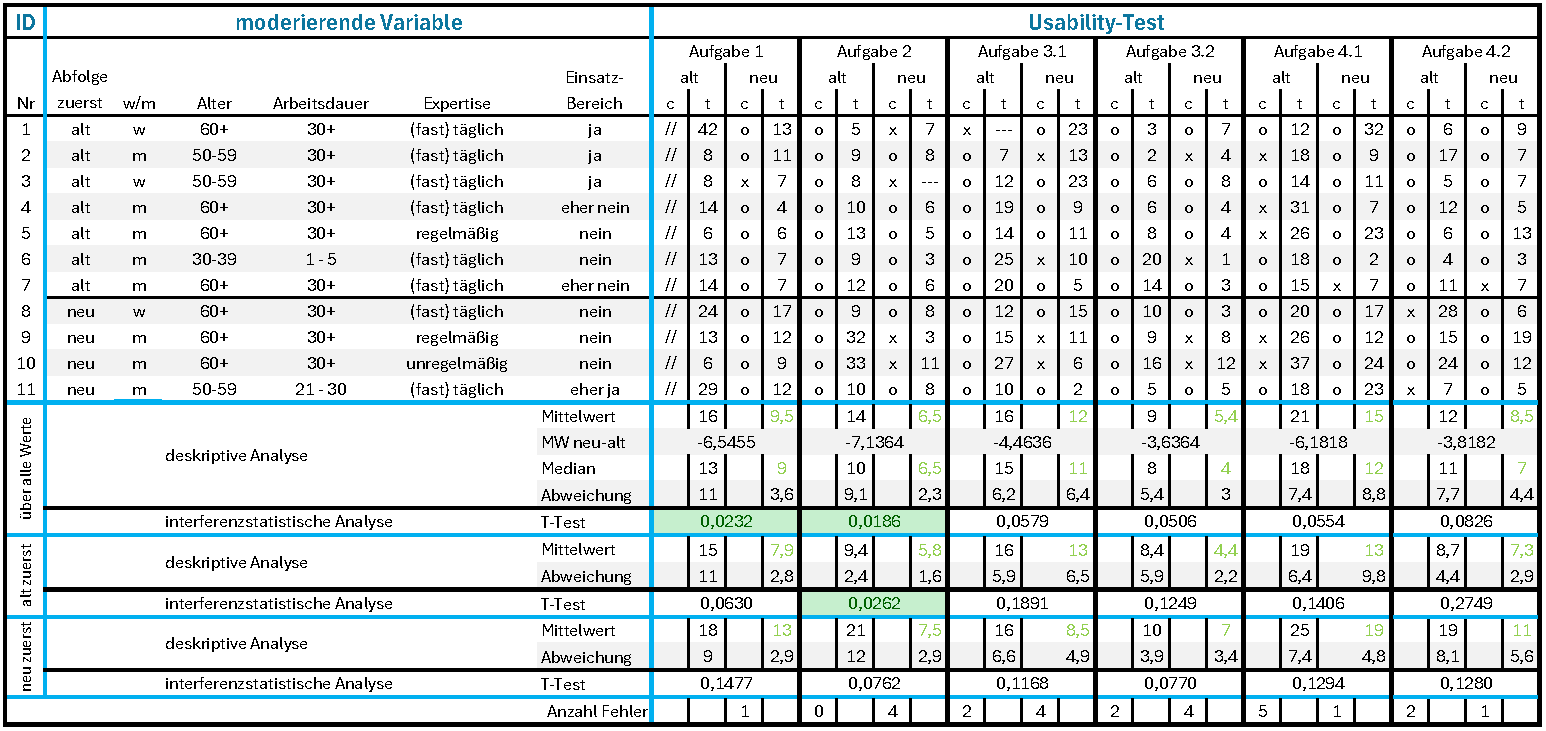
\includegraphics[width=0.85\textheight, angle=90]{Anhänge/05_Usability-Test/UT_rohe_Daten.pdf}
    \caption{aufgezeichnete Daten des Usability-Tests}
    \label{tab:Usability_Test:rohe_Daten}
\end{table}

% *********************************************************************************

\begin{table}[H]
\justifying
\begin{tabular}{|l|c|c|c|c|}
\hline
Aufgabe 1\textcolor{white}{.0}   & $\Bar{x}$ & $\Tilde{x}$ & $\sigma$ & f \\ \hline
alt                              & 16        &  13         &  11      &  0\%   \\ \hline
neu                              & 9,5       &  9          &  3,6     &  9,09\%   \\ \hline
%Differenz   &           &             & -     &  xxx   \\ \hline
%\end{tabular}
%\begin{tabular}{|l|c|c|c|c|}
\hline
Aufgabe 2\textcolor{white}{.0}   & $\Bar{x}$ & $\Tilde{x}$ & $\sigma$ & f \\ \hline
alt                              & 14        &  10         &  9,1  &  0\%   \\ \hline
neu                              & 6,5       &  6,5        &  2,3  &  30\%   \\ \hline
%Differenz   &           &             & -     &  xxx   \\ \hline
%\end{tabular}
%\begin{tabular}{|l|c|c|c|c|}
\hline
Aufgabe 3.1   & $\Bar{x}$ & $\Tilde{x}$ & $\sigma$ & f \\ \hline
alt           & 16        &  15         &  6,2  &  0\%   \\ \hline
neu           & 12        &  11         &  6,4  &  36,36\%   \\ \hline
%Differenz   &           &             & -     &  xxx   \\ \hline
\end{tabular}
\begin{tabular}{|l|c|c|c|c|}
\hline
Aufgabe 3.2   & $\Bar{x}$ & $\Tilde{x}$ & $\sigma$ & f \\ \hline
alt           & 9         &  8          &  5,4  &  0\%   \\ \hline
neu           & 5,4       &  4          &  3    &  36,36\%   \\ \hline
%Differenz   &           &             & -     &  xxx   \\ \hline
%\end{tabular}
%\begin{tabular}{|l|c|c|c|c|}
\hline
Aufgabe 4.1   & $\Bar{x}$ & $\Tilde{x}$ & $\sigma$ & f \\ \hline
alt           & 21        &  18         &  7,4  &  45,45\%   \\ \hline
neu           & 15        &  12         &  8,8  &  9,09\%   \\ \hline
%Differenz   &           &             & -     &  xxx   \\ \hline
%\end{tabular}
%\begin{tabular}{|l|c|c|c|c|}
\hline
Aufgabe 4.2   & $\Bar{x}$ & $\Tilde{x}$ & $\sigma$ & f \\ \hline
alt           & 12        &  11         &  7,7  &  18,18\%   \\ \hline
neu           & 8,5       &  7          &  4,4  &  9,09\%   \\ \hline
%Differenz   &           &             & -     &  xxx   \\ \hline
\end{tabular}

\begin{tabular}{ll}
\multicolumn{2}{l}{verwendete Formelzeichen:} \\ \hline
$\Bar{x}$          & Mittelwert               \\
$\Tilde{x}$        & Median                   \\
$\sigma$           & Standardabweichung       \\
f                  & Fehlerquote
\end{tabular}
\caption{Zusammenfassung der Ergebnisse des Usability-Tests (Weiterverarbeitung der Daten aus \autoref{tab:Usability_Test:rohe_Daten})}
\label{tab:usability_test:mittelwerte}
\end{table}

% *********************************************************************************

\begin{table}[H]
    \centering
    \begin{tabular}{|l|c|c|c|c|c|c|}
    \hline
    Aufgabe                                     & 1     & 2     & 3.1   & 3.2     & 4.1   & 4.2 \\ \hline
    $\varnothing t_{neu} - \varnothing t_{alt}$ & -6,55 & -7,14 & -4,46 & -3,64 & -6,18 & -3,81 \\ \hline
    t-Test                                      & 0,0231& 0,0186& 0,0579& 0,0506& 0,0554& 0,0826\\ \hline
    \end{tabular}
    
    \caption{Usability Test - Differenz der Zeitmittelwerte und t-Test-Ergebnisse (Weiterverarbeitung der Daten aus \autoref{tab:usability_test:mittelwerte})}
    \label{tab:usability_test:Differenz+ttest_Zeit}
\end{table}

\begin{table}[H]
    \centering
    \begin{tabular}{|l|c|c|c|c|c|c|c|c|}
    \hline
     & 1      & 2    & 3.1     & 3.2     & 4.1     & 4.2     & $\varnothing$ & t-Test                  \\ \hline
    alt     & 0\%    & 0\%  & 0\%     & 0\%     & 45,45\% & 18,18\% & 10,61\% & \multirow{2}{*}{0,1989} \\ \cline{1-8}
    neu     & 9,09\% & 30\% & 36,36\% & 36,36\% & 9,09\%  & 9,09\%  & 21,67\% &                         \\ \hline
    \end{tabular}
    \caption{Usability Test - Fehlerquoten, -mittelwerte und t-Test-Ergebnisse (Weiterverarbeitung der Daten aus \autoref{tab:usability_test:mittelwerte})}
    \label{tab:usability_test:Differenz+ttest_Fehler}
\end{table}  % fig:Usability-Test:Excel_Berechnungen

\begin{table}[H]
    \centering
    \begin{tabular}{|l|c|c|c|c|c|c|c|}
        \hline
            & 1 & 2 & 3.1 & 3.2 & 4.1 & 4.2 & tTest \\ \hline
        alt	& 16,0909 & 13,6364 & 16,1 & 9 & 39,16667 & 15 & \multirow{2}{*}{0,0720} \\ \cline{1-7}
        neu	& 10,5 & 9,2857 & 18,2857 & 8,4286 & 16,7 & 9,3	& \\ \hline
        Verhältnis* & 53,25\% & 46,85\% & -11,95\% & 6,78\% & 134,53\% & 61,29\% & 0,0336 \\ \hline
    \end{tabular}
    \caption{Usability-Test - Effizienzbewertung der Systeme im Verhältnis zueinander (Weiterverarbeitung der Daten aus \autoref{tab:Usability_Test:rohe_Daten} anhand der \nameref{Formel_zur_Effizienzberechnung})}
    \textcolor{white}{.}\hfill *Dashboard im Vergleich zum alten System
    \label{tab:usability_test:effizienz}
\end{table}
